\chapter{Particle in a Central Potential. The Hydrogen Atom}\sn{Quantum Mechanics - Cohen-Tannoudji, Diau, Laloe.}
In this chapter, we shall consider the quantum mechanical properties of a particle placed in a central potential [that is, a potential $V(r)$ which depends only on the distance $r$ from the origin]. This problem is closely related to the study of angular momentum. As we shall know, the fact that $V(r)$ es invariant under any rotation about the origin means that the Hamiltonian $H$ of the particle conmutes with the three components of the orbital angular momentum operator $\vb{L}$. This cosiderably simplifies the determination of the eigenfunctions and eigenvalues of $\vb{L}^2$ and $L_z$ as well.



\section{Statioanary states of a particle in a central potential}\label{sec:A}
In this section, we consider a (spinless) particle of mass $\mu$, subjected to a central force derived from the potential $V(r)$ (the center of force is chosen as the origin).
\subsection{Outline of the problem}
\subsubsection{Review of some classical results}
The force acring on the classical particle situated at the point $M$ (with $\vb{OM}=\vb{r}$) is equal to:
\begin{equation}\label{A-1}
	\vb{F}=-\nabla V(r)=-\dv{V}{r}\frac{\vb{r}}{r}
\end{equation}
$\vb{F}$ is always directed towards $O$,  and its mimentum with respect to this point is therefore always zero. If:
\begin{equation}\label{A-2}
	\vb{\mathcal{L}}=\vb{r}\times\vb{p}
\end{equation}
is the angular momentum of the particle with respecto to $O$, the anfular momentum theorem implies that:
\begin{equation}\label{A-3}
	\dv{\vb{\mathcal{L}}}{t}=\vb{0}
\end{equation}
$\vb{\mathcal{L}}$ is therefore a \textit{constant of the motion}, so that the particle's trajectory is necessarily situated in the plane passing through $O$ and perpendicular to $\vb{\mathcal{L}}$.

\begin{figure}[h]
	\begin{center}
		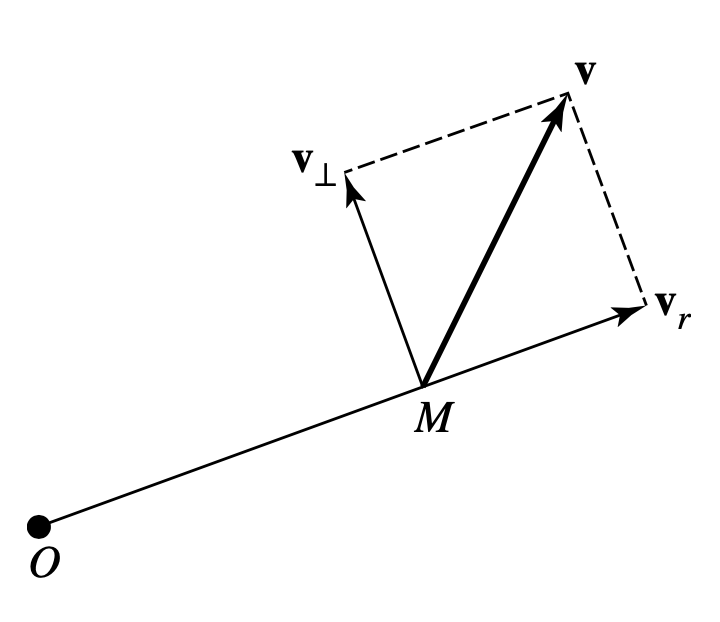
\includegraphics[scale=0.6]{fig/fig1-A-cohen.png}
		\caption{Radial component $\vb{v}_r$ and tangential component $\vb{v}_\perp$ of a particle's velocity.}
		\label{fig:1-a-cohen}
	\end{center}	
\end{figure}

Now let us consider Fig. \ref{fig:1-a-cohen} the position (denoted by $\vb{OM}=\vb{r}$) and velocity $\vb{v}$ of the particle at the instant $t$. Thw two vectors $\vb{r}$ and $\vb{v}$ lie in the plane of the trajectory and the velocity $\vb{v}$ can be decomposed into the radial component $\vb{v}_r$ (along the axis defined by $\vb{r}$) and the tangential component $\vb{v}_\perp$ (along the axis perpendicular to $\vb{r}$). The radual velocity, the algebraic value of $\vb{v}_r$, is the time derivative of the distance of the particle from the point $O$:
\begin{equation}\label{A-4}
	v_r=\dv{r}{t}
\end{equation}
The tangential velociry can be expressed in term of $r$ and the angular momentum $\vb{\mathcal{L}}$, since:
\begin{equation}\label{A-5}
	|\vb{r}\times\vb{v}|=r|\vb{v}_\perp|
\end{equation}
so that the modulus of the angular momentum $\vb{\mathcal{L}}$ is equal to:
\begin{equation}\label{A-6}
	|\vb{\mathcal{L}}|=|\vb{r}\times\mu\vb{v}|=\mu r|\vb{v}_\perp|
\end{equation}
The total energy of the particle:
\begin{equation}\label{A-7}
	E=\frac{1}{2}\mu\vb{v}^2+V(r)=\frac{1}{2}\mu \vb{v}_r^2+\frac{1}{2}\mu \vb{v}_\perp^2+V(r)
\end{equation}
can be written:
\begin{equation}\label{A-8}
	E=\frac{1}{2}\mu\vb{v}_r^2+\frac{\vb{\mathcal{L}}^2}{2\mu r^2}+V(r)
\end{equation}
The classical Hamiltonian if the system is then:
\begin{equation}\label{A-9}
	\mathcal{H}=\frac{p_r^2}{2\mu}+\frac{\vb{\mathcal{L}}^2}{2\mu r^2} + V(r)
\end{equation}
where:
\begin{equation}\label{A-10}
	p_r=\mu\dv{r}{t}
\end{equation}
is the conjugate momentum of $r$,  and $\vb{\mathcal{L}}^2$ must be expressed in terms of the variables $r, \theta, \varphi$ and their conjugate momenta $p_r,p_\theta,p_\varphi$. One finds:
\begin{equation}\label{A-11}
	\vb{\mathcal{L}}^2=p_\theta ^2 +\frac{1}{\sin^2\theta}p_\varphi^2
\end{equation}
In expression (\ref{A-9}), the kinetic energy is broken into two terms: the radial kinetic energy and the kinetic energy of rotation about $O$ . The reason is that, since $V(r)$ is independent of $\theta$ and $\varphi$ in this case, the angular variables and their conjugate momenta appear only in the $\vb{\mathcal{L}}^2$ term. In fact, if we are interested in the evolution of $r$, we can use the fact that $\vb{\mathcal{L}}$ is a constant of the motion, and replace $\vb{\mathcal{L}}^2$ by a constant in expression (\ref{A-9}). The Hamiltonian $\mathcal{H}$  then appears as a function only of the radial variables $r$ and $p_r$ ( $\vb{\mathcal{L}}^2$ plays the role of a parameter), and the result is a differential equation involving only one variable, $r$:
\begin{equation}\label{A-12a}
	\dv{p_r}{t}=\mu\dv[2]{r}{t}=-\pdv{\mathcal{H}}{r}
\end{equation}
that is:
\begin{equation}\label{A-12b}
	\mu\pdv[2]{r}{t}=\frac{\vb{\mathcal{L}}^2}{\mu r^2}-\dv{V}{r}
\end{equation}
It is just as if we had a one-dimensional problem (with $r$ varyng only between $0$ and $+\infty$), with a particle of mass $\mu$ subjected to the "efective potential":
\begin{equation}\label{A-13}
	V_{eff}(r)=V(r)+\frac{\vb{\mathcal{L}}^2}{2\mu r^2}
\end{equation}
We shall see that the situation is analogous in quantum mechanics.


\subsubsection{The quantum mechanical Hamiltonian}
In quantum mechanics, we want to solve the eigenvalue equation of the Hamiltonian $\mathcal{H}$, the observable associated with the total energy. This equation is written, in the $\{\ket{\vb{r}}\}$ representation:
\begin{equation}\label{A-14}
	\left[-\frac{\hbar^2}{2\mu}\Delta +V(r)\right]\varphi(\vb{r}) = E\varphi(\vb{r})
\end{equation}
Since the potential $V$ depends only on the distance  $r $of the particle from the origin, spherical coordinates are best adapted to the problem. We therefore express the Laplacian $\Delta$ in spherical coordinates \sn{Expression (\ref{A-15}) gives the Laplacian only for non-zero $r$. This is because of the privileged position of the origin in spherical coordinates; it can be seen, moreover, that expression (\ref{A-15}) is not defined for $r=0$.}
\begin{equation}\label{A-15}
	\Delta = \frac{1}{r}\pdv[2]{r}r+\frac{1}{r^2}\left(\pdv[2]{\theta} +\frac{1}{\tan\theta}\pdv{\theta}+\frac{1}{\sin^2\theta}\pdv[2]{\varphi}\right)
\end{equation}
and look for eigenfucntions $\varphi(\vb{r})$ that are functions of the variables $r,\theta,\varphi$.

If we compare expression (\ref{A-15}) with the one for the operator $\vb{\mathcal{L}}^2$, wee see that the quantum mechanical Hamiltonian $\mathcal{H}$ can be put in a form completely analogous to (\ref{A-9}):
\begin{equation}\label{A-16}
	\boxed{H=-\frac{\hbar^2}{2\mu}\frac{1}{r}\pdv[2]{r}+\frac{1}{2\mu r^2}\vb{L}^2+V(r)}
\end{equation}
The angular dependence of the Hamiltonian is contained entirely in the $\vb{L}^2$ term, which is an operator here. We could, in fact, perfect the analogy by defining an operator $P_r$, which would allow us to write the first term of (\ref{A-16}) like the one in (\ref{A-9}).

We shall now show how one can solve the eigenvalue equation:
\begin{equation}\label{A-17}
	\left[-\frac{\hbar^2}{2\mu}\frac{1}{r}\pdv[2]{r}+\frac{1}{2\mu r^2}\vb{L}^2+V(r)\right]\varphi(r,\theta,\varphi)=E\varphi(r,\theta,\varphi)
\end{equation}

\subsection{Separation of variables}
\subsubsection{Angular dependence of the eigenfunctions}
We know that the three components of the angular momentum operator $\vb{L}$ act only on the angular variables $\theta$ and $\varphi$ ; consequently, they commute with all operators acting only on the $r$-dependence. In addition, they commute with $\vb{L}^2$. Therefore, according to expression (\ref{A-16}) for the Hamiltonian, \textit{the three components of L are constants of the motion\sn{(\ref{A-18}) express the fact that $H$ is a scalar operator with respect to rotations about the point $O$. This is true because the potential energy is invariant under rotations about $O$.}} in the quantum mechanical sense:
\begin{equation}\label{A-18}
	[H,\vb{L}]=\vb{0}
\end{equation}

Obviously, $H$ also commutes with $\vb{L}^2$.

Although we have at our disposition four constants of the motion ($L_x,L_y,L_z$ and $\vb{L}^2$), we cannot use all four of them to solve equation (\ref{A-17}) because they do not commute with each other; we shall use only $\vb{L}^2$ and $L_z$. Since the three observables $H$, $\vb{L}^2$ and $L_z$ commute, we can find a basis of the state space $\mathcal{E}_r$ of the particle composed of eigenfunctions common to these three observables. We can, therefore,  require the functions $\varphi(r,\theta,\varphi)$, solutions of equation (\ref{A-17}), to be eigenfunctions of $\vb{L}^2$ and $L_z$  as well. We must then solve the system of differential equations:
\begin{align}
	\label{A-19a}H\varphi(\vb{r})&=E\varphi(\vb{r})\\
	\label{A-19b}\vb{L}^2\varphi(\vb{r})&=l(l+1)\hbar^2\varphi(\vb{r})\\
	L_z\varphi(\vb{r})&=m\hbar \varphi(\vb{r}) \label{A-19c}
\end{align}
But we already know the general form of the common eigenfunctions of $\vb{L}^2$ and $L_z$: the solutions $\varphi(\vb{r})$ of equations (\ref{A-19a}), (\ref{A-19b}), (\ref{A-19c}) corresponding to fixed values $l$ of and $m$ , are necessarily products of a function of $r$ alone and the spherical harmonic $Y_l^m(\theta,\varphi)$:
\begin{equation}\label{A-20}
	\varphi(\vb{r})=R(r)Y_l^m(\theta,\varphi)
\end{equation}
Whatever the radial function $R(r)$, $\varphi(\vb{r})$ is a solution of equations (\ref{A-19b}) and (\ref{A-19c}). The only problem which remains to be solved is therefore how to determine $R(r)$ such that $\varphi(\vb{r})$ is also an eigenfunction of $H$ [equation (\ref{A-19a})].

\subsubsection{The radial equation}
We shall now substitute expressions (\ref{A-16}) and (\ref{A-20}) into (\ref{A-19a}). Since $\varphi(\vb{r})$ is an eigenfunction of $\vb{L}^2$ with the eigenvalue $l(l+1)\hbar^2$, we see that $Y_l^m(\theta,\varphi)$ is a common factor on both sides. After simplifyng, we obtain the radial equation:
\begin{equation}\label{A-21}
	\left[-\frac{\hbar^2}{2\mu}\frac{1}{r}\dv[2]{r}r+\frac{l(l+1)\hbar^2}{2\mu r^2}+V(r)\right]R(r)=ER(r)
\end{equation}
Actually, a solution of (\ref{A-21}), substituted into (\ref{A-20}), does not necessarily yield a solution of the eigenvalue equation (\ref{A-14}) of the Hamiltonian. As we have already pointed out, expression (\ref{A-15}) for the Laplacian is not necessarily valid at $r=0$. We must therefore make sure that the behavior of the solutions $R(r$) of (\ref{A-21}) at the origin is sufficiently regular for (\ref{A-20}) to be in fact a solution of (\ref{A-14}).

Instead of solving the partial differential equation (\ref{A-17}) involving the three variables $r,\theta\varphi$ we must now solve a differential equation involving only the variable $r$, but dependent on a parameter $l$: we are looking for eigenvalues and eigenfunctions of an operator $H_l$ which is different for each value of $l$.

In other words, we consider separately, in the state space $\mathcal{E}_r$, the subspaces $\mathcal{E}(l,m)$ corresponding to fixed values of $l$ and $m$ , studying the eigenvalue equation of $H$ in each of these subspaces (which is possible because $H$ commutes with $\vb{L}^2$ and $L_z$). The equation to be solved depends on $l$ , but not on $m$ ; it is therefore the same in the $(2l+1)$ subspaces $\mathcal{E}(l,m)$ associated with a given value of $l$. We shall denote by $_{k,l}$ the eigenvalues of $H_l$ , that is, the eigenvalues of the Hamiltonian $H$ inside a given subspace $\mathcal{E}(l,m)$. The index $k$, which can be discrete or continuous, represents the various eigenvalues associated with the same value of $l$. As for the eigenfunctions of $H_l$, we shall label them with the same two indices as the eigenvalues: $R_{k,l}(r)$. It is not obvious that this is sufficient: several radial functions might exist and be eigenfunctions of the same operator $H_l$ with the same eigenvalue $E_{k,l}$; we shall see that this is not the case and that, consequently, the two indices $k $and $l$ are sufficient to characterize the different radial functions. We shall therefore rewrite equation (\ref{A-21}) in the form:
\begin{equation}\label{A-22}
	\left[-\frac{\hbar^2}{2\mu}\frac{1}{r}\dv[2]{r}+\frac{l(l+1)\hbar^2}{2\mu r^2}+V(r)\right]R_{k,l}(r)=E_{k,l}R_{k,l}(r)
\end{equation}
We can simplify the differential operator to be studied by a change in functions.

We set:
\begin{equation}\label{A-23}
	R_{k,l}(r)=\frac{1}{r}u_{k,l}(r)
\end{equation}
Multiplying both sides of (\ref{A-22}) by $r$, we obtain for $u_{k,l}(r)$ the following differential equation:
\begin{equation}\label{A-24}
	\boxed{\left[-\frac{\hbar^2}{2\mu}\dv[2]{r}+\frac{l(l+1)\hbar^2}{2\mu r^2}+V(r)\right]u_{k,l}(r)=E_{k,l}(r)u_{k,l}(r)}
\end{equation}
This equation is analogous to the one we would have to solve if, in a \textit{one-dimensional} problem, a particle of mass $\mu$ were moving in an \textit{effective potential} $V_{eff}(r)$: 
\begin{equation}\label{A-25}
	V_{eff}(r)=V(r)+\frac{l(l+1)\hbar^2}{2\mu r^2}
\end{equation}
Nevertheless, we must not lose sight of the fact that the variable $r$ can take on only \textit{non-negative} real values. The term $l(l+1)\hbar^2/2\mu r^2$ which is added to the potentual $V(r)$ is always positive or zero; the corresponding force (equal to minus the gradient of this term) always tend to repel the particle from the force center $O$; this is whay this term is called the \textit{centrifugal potential} (or centrifugal barrier).

\subsubsection{Behavior of the solutions of the radial equation at the origin}\label{sec:A-2-c}
We have already pointed out that it is necessary to examine the behavior of the solutions $R(r)$ of the radial equation (\ref{A-21}) at the origin in order to know if they are really solutions of (\ref{A-14}).

We shall assume that when $r$ approaches zero, the potential $V(r)$ remains finite, or at least approaches infinity less rapidly than $1/r$ (this hypothesis is true in most cases encountered in physics and, in particular, in the case of the Coulomb potential. We shall consider a solution of (\ref{A-22}) and assume that it behaves at the origin like $r^s$:
\begin{equation}\label{A-26}
	R_{k,l}(r)\thicksim Cr^s\quad \mbox{,as } r\to 0
\end{equation}
Substituting (\ref{A-26}) into (\ref{A-22}), and setting the coefficient of the dominant term equal to zero, we obtain the equation:
\begin{equation}
	-s(s+1) + l(l+1)=0
\end{equation}
and, consequently:

\begin{equation}\label{A-28}
	\left \{
		\begin{array}{ccc}
			\mbox{either} & s=l\\
			\mbox{or}  & s=-(l+1)
		\end{array}
	\right.
\end{equation}

For a given value of $E_{k,l}$, there are therefore two linearly independent solutions of the second-order equation (\ref{A-22}), behaving at the origin like $r^l$ and $1/R^{l+1}$, respectively. But those which behave like $1/r^{l+1}$ must be rejected, since it can be shown\sn{This is because the Laplacian of $\frac{1}{r^{l+1}}Y_l^m(\theta,\varphi)$ involves the $l$th derivatives of $\delta(\vb{r})$.} that $\frac{1}{r^{l+1}}Y_l^m(\theta,\varphi)$ is not a solution of the eigenvalue equation (\ref{A-14}) for $r=0$. From this, we see that acceptable solution of (\ref{A-24}) go to zero at the origin for all $l$, since:
\begin{equation}\label{A-29}
	u_{k,l}(r)\thicksim Cr^{l+1}\quad  \mbox{,as } r\to 0
\end{equation}
Consequantly, to (\ref{A-24}) must be added the condition:
\begin{equation}\label{A-30}
	\boxed{u_{k,l}(0)=0}
\end{equation}

\subsection{Statioanary states of a particle in a central potential}
\subsubsection{Quantum numbers}
We can summarize the results as follows: the fact that the potential $V(r)$ is independent of $\theta$ and $\varphi$ makes it possible:
\begin{enumerate}
	\item to require the eigenfunctions of $H$ to be \textit{simultaneous eigenfunctions} of $\vb{L}^2$ \textit{and} $L_z$, \textit{which determines their angular dependence}:
		\begin{equation}\label{A-31}
	\varphi_{k,l,m}(\vb{r})=R_{k,l}(r)Y_l^m(\theta,\varphi)=\frac{1}{r}u_{k,l}(r)Y_l^m(\theta,\varphi)
\end{equation}
\item \textit{to replace the eigenvalue equation of} $H$, an equation involving partial derivatives with respect to $r,\theta,\varphi$ by a \textit{differential equation involving only the variable} $r$ and depending on a parameter $l$ [(\ref{A-24})], with condition (\ref{A-30}) imposed.
\end{enumerate}

In principle, the functions $\varphi_{k,l,m}(r,\theta,\varphi)$ must be squre-integrable, that is, normalizable:
\begin{equation}\label{A-32}
	\int |\varphi_{k,l,m}(r,\theta,\varphi)|^2r^2\dd r\dd \Omega = 1
\end{equation}
Their form (\ref{A-31}) allows us to separate radial and angular integrations:
\begin{equation}\label{A-33}
	\int |\varphi_{k,l,m}(r,\theta,\varphi)|^2r^2\dd r\dd \Omega =\int_0^\infty r^2\dd r R_{k,l}(r)|^2\int \dd\Omega |Y_l^m(\theta,\varphi)|^2
\end{equation}
But the spherical harmonics $Y_l^m(\theta,\varphi)$ are normalized with respect to $\theta$ and $\varphi$; condition (\ref{A-32}) therefore reduces to:
\begin{equation}\label{A-34}
	\int_0^\infty r^2\dd r |R_{k,l}(r)|^2=\int_0^\infty \dd r |u_{k,l}(r)|^2=1
\end{equation}
Actually, we know that it is often convenient to accept eigenfunctions of the Hamil- tonian that are not square-integrable. If the spectrum of $H$ has a continuous part, we shall require only that the corresponding eigenfunctions be orthonormalized in the ex- tended sense, that is, that they satisfy a condition of the form:
\begin{equation}\label{A-35}
	\int_0^\infty r^2\dd r R_{k,l}^*(r)R_{k,l}(r)=\int_0^\infty \dd r u_{k,l}^*(r)u_{k,l}(r)=\delta(k'-k)
\end{equation}
where $k$ is a continuous index.
In (\ref{A-34}) and (\ref{A-35}), the integrals converge at their lower limit, $r=0$ [condition (\ref{A-30})]. This is physically satisfying since the probability of finding the particle in any volume of finite dimensions is then always finite. It is therefore only because of the behavior of the wave functions for $r\to \infty$ that, in the case of a continuous spectrum, the normalization integrals (\ref{A-35}) diverge if $k=k'$.

Finally, the eigenfunctions of the Hamiltonian $H$ of a particle placed in a central potential $V(r)$ depend on at least three indices [formula (\ref{A-31})]: $\varphi_{k,l,m}(r,\theta,\varphi)=R_{k,l}(r)Y_l^m(\theta,\varphi)$ is a somultaneous eigenfunction of $H, \vb{L}^2$ and $L_z$ with the respective eigenvalues $E_{k,l}, l(l+1)\hbar^2$ and $m\hbar$. $k$ is called the \textit{radial} quantum number; $l$, the \textit{azimuthal} quantum number; and $m$ the \textit{magnetic} quantum number. The radial part $R_{k,l}(r)=\frac{1}{r}u_{k,l}(r)$ of the eigenfunction and the eigenvalue $E_{k,l}$ of $H$ are independent of the magnetic quantum number and are given by the radial equation (\ref{A-24}). The angular part of the eigenfunction depends only on $l$ and $m$ and not on $k$; it does not depend on the form of the potentual $V(r)$.

\subsubsection{Degeneracy of the energy levels}

\section{Potion of the center of mass and relative motion for a system fo two interacting particles}

\subsection{Motion od the center of masss and relative motion in classical mechanics}

\subsection{Separation of variables in quantum mechanics}
\subsubsection{Eigenvalues and eigenfunctions of the Hamiltonian}

\section{The hydrogen atom}
\subsection{Introduction}
The hydrogen atom consists of a proton, of mass:
\begin{equation}\label{C-1}
	m_p\approx 1.7\times 10^{-27} \mbox{ kg}
\end{equation}
and charge:
\begin{equation}\label{C-2}
	q\approx 1.6\times 10^{-19} \mbox{ Coulomb}
\end{equation}
and of and electron, of mass:
\begin{equation}\label{C-3}
	m_e\approx 0.91\times 10^{-30}\mbox kg
\end{equation}
and a charge $-q$. The interaction between these two particles is essentially electrostatic. The corresponding potential energy is:
\begin{equation}\label{C-4}
	V(r)\approx -\frac{q^2}{4\pi\epsilon_0}\frac{1}{r}=-\frac{e^2}{r}
\end{equation}
where $r$ denotes the distance between the two particles, and:
\begin{equation}\label{C-5}
	\frac{q^2}{4\pi\epsilon_0}=e^2
\end{equation}
We confine ourselves to the study of this system in the center of mass frame. The classical Hamiltonian that describes the relative motion of the two particles is then:
\begin{equation}\label{C-6}
	\mathcal{H}(\vb{r},\vb{p})=\frac{\vb{p}^2}{2\mu}-\frac{e^2}{r}
\end{equation}
Since $m_p \gg m_e$ [formulas (\ref{C-1}) and (\ref{C-3})], the reduced mass $\mu$ of the system is very close to $m_e$:
\begin{equation}\label{C-7}
	\mu=\frac{m_em_p}{m_e+m_p}\approx m_e\left(1-\frac{m_e}{m_p}\right)
\end{equation}
(the correction term $m_e/m_p$ is on the order of $1/1800$).  This means that the center of mass of the system is practically at the position of the proton, and that the relative particle can be identified, to a very good approximation, with the electron. This is why we shall adopt the slightly inaccurate convention of calling the relative particle the electron and the center of mass the proton.

\subsection{The Bohr model}
We shall briefly review the results of the Bohr model, which relate to the hydrogen atom. This model, which is based on the concept of a trajectory, is incompatible with the ideas of quantum mechanics. However, it allows us to introduce, in a very simple way, fundamental quantities such as the ionization energy $E_I$ of the hydrogen atom and a parameter which characterizes atomic dimensions (the Bohr radius $a_0$). In addition, it so happens that the energies $E_n$ given by the Bohr theory are the same as the eigenvalues of the Hamiltonian we shall calculate in \ref{sec:C-3}. Finally, quantum mechanical theory is in agreement with some of the intuitive images of the Bohr model.

This semi-classical model is based on the hypotesis that the electron describes a \textit{circular orbit} of radius $r$ about the proton, obeying the following equations:
\begin{align}
	\label{C-8}E&=\frac{1}{2}\mu v^2-\frac{e^2}{r}\\
	\label{C-9}\frac{\mu v^2}{r}&=\frac{e^2}{r^2}\\
	\mu  v r&=n\hbar\quad ; \quad \mbox{$n$ a positive number}\label{C-10}
\end{align}
The first two equations are classical ones. (\ref{C-8}) expresses the fact that the total energy $E$ of the electron is the sum of its kinetic energy $\mu v^2/2$  and its potential energy $-e^2/r$ . (\ref{C-9}) is none other than the fundamental equation of Newtonian dynamics ($e^2/r^2$ is the Coulomb force exerted on the electron, and $v^2/r$ is the acceleration of its uniform circular motion). The third equation expresses the quantization condition, introduced empirically by Bohr in order to explain the existence of discrete energy levels: he postulated that only circular orbits satisfying this condition are possible trajectories for the electron. The different orbits, as well as the corresponding values of the various physical quantities, are labeled by the integer $n$ associated with them.

A very simple algebraic calculation then yields the expressions for $E_n,r_n$ and $v_n$:
\begin{align}
	\label{C-11a}E_n&=-\frac{1}{n^2}E_I\\
	\label{C-11b}r_n&=n^2a_0\\
	v_n&=\frac{1}{n}v_0\label{C-11c}
\end{align}
with 
\begin{align}
	\label{C-12a}E_I&=\frac{\mu e^4}{2\hbar^2}\\
	\label{C-12b}a_0&=\frac{\hbar^2}{\mu e^2}\\
	v_0&=\frac{e^2}{\hbar}\label{C-12c}
\end{align}
When this model was proposed by Bohr, it marked an important step towards the understanding of atomic phenomena, since it yielded the correct values for the energy level of the hydrogen atom. These values indeed follow the $1/n^2$ (the Balmer formula) law indicated by expression (\ref{C-11a}). Moreover, the experimentally measured \textit{ionization energy} (the energy which must be supplied to the hydrogen atom in its ground state in order to remove the electron) is equal to the numerical value of $E_I$:
\begin{equation}\label{C-13}
	E_I\approx 13.6 \mbox{ eV }
\end{equation}
Finally, the \textit{Bohr radius} $a_0$ indeed characterized atomix¡c dimensions:
\begin{equation}\label{C-14}
	a_0\approx 0.52  \,\si{\angstrom}
\end{equation}

\subsection{Quantum mechanical theory of the hydrogen atom}\label{sec:C-3}
We shall now take up the question of the determination of the eigenvalues and eigenfunctions of the Hamiltonian $H$ describing the relative motion of the proton and
the electron in the center of mass frame [formula (\ref{C-6})]. In the $\{\ket{\vb{r}}\}$ representation, the eigenvalue equation of the Hamiltonian $H$ is written:
\begin{equation}\label{C-15}
	\left[-\frac{\hbar^2}{2\mu}\Delta -\frac{e^2}{r}\right]\varphi(\vb{r})=E\varphi(\vb{r})
\end{equation}
Since the potential $-e^2/r$ is central, we can apply the results of \ref{sec:A}: the eigenfunctions $\varphi(\vb{r})$ are of the form:
\begin{equation}\label{C-16}
	\varphi_{k,l,m}(\vb{r})=\frac{1}{r}u_{k,l}(r)Y_l^m(\theta,\varphi)
\end{equation}
$u_{k,l}(r)$ is given by the radial equation, (\ref{A-24}), that is:
\begin{equation}\label{C-17}
	\left[-\frac{\hbar^2}{2\mu}\dv[2]{r}+\frac{l(l+1)\hbar^2}{2\mu r^2}-\frac{e^2}{r}\right]u_{k,l}(r)=E_{k,l}(r)u_{k,l}(r)
\end{equation}
We add to this equation condition (\ref{A-30}):
\begin{equation}\label{C-18}
	u_{k,l}(0)=0
\end{equation}

\subsubsection{Change of variables}
To simplify the reasoning, we shall choose $a_0$ and [formulas (\ref{C-12a}), (\ref{C-12b}) and (\ref{C-12c})] as the units of length and energy. That is, we shall introduce the dimensionless quantities:
\begin{equation}\label{C-19}
	\rho = r/a_0
\end{equation}
\begin{equation}\label{C-20}
	\lambda_{k,l}=\sqrt{-E_{k,l}/E_I}
\end{equation}
(the quantity under the radical sign is positive, since we are looking for the bound states).

With expressions (\ref{C-12a}) and (\ref{C-12b}) for $E_I $and $a_0$ taken into account, the radial equation (\ref{C-17}) becomes simply:
\begin{equation}\label{C-21}
	\left[\dv[2]{\rho}-\frac{l(l+1)}{\rho^2}+\frac{2}{\rho}\right]u_{k,l}(\rho)=0
\end{equation}

\subsubsection{Solving the radial equation}
In order to solve (\ref{C-21}), we shall expanding $u_{k,l}(\rho)$ in a power series.

\begin{itemize}
	\item Asymptotic behavior

		Let us determine the asymptotic behavior of $u_{k,l}(\rho)$ qualitatively. When $\rho$ approaches infinity, the terms in $1/\rho$ and $1/\rho^2$ become negligible compared to the constant term $\lambda_{k,l}^2$, so that (\ref{C-21}) practically reduces to:
		\begin{equation}\label{C-22}
			\left[\dv[2]{\rho}-\lambda_{k,l}^2\right]u_{k,l}(\rho)=0
\end{equation}
whose solutions are $e^{\pm\rho\lambda_{k,l}}$. This argument is not rigorous, since we have completely neglected the terms in $1/\rho$ and $1/\rho^2$; actually, it can be shown that $u_{k,l}(\rho)$ is equal to $E^{\pm\rho\lambda_{k,l}}$ multiplied by a power of $\rho$.

We shall later be led by physical considerations to require the function $u_{k,l}(\rho)$ to be bounded at infinity, and hence to reject the solutions of (\ref{C-21}) whose asymptotic behavior is governed by $e^{+\rho\lambda_{kl}}$ . This is why we perform the change of function:
\begin{equation}\label{C-23}
	u_{k,l}(\rho)=e^{-\rho\lambda_{k,l}}y{k,l}(\rho)
\end{equation}
Although this change of function singles out $e^{-\rho\lambda_{k,l}}$ , it clearly does not eliminate solutions in $e^{+\rho\lambda_{k,l}}$ , which must be identified and then rejected at the end of the calculation. The differential equation that $y_{k,l}(\rho)$ must satisfy can easily be derived from (\ref{C-21}):
\begin{equation}\label{C-24}
	\left\{\dv[2]{\rho}-2\lambda_{k,l}\dv{\rho}+\left[\frac{2}{\rho}-\frac{l(l+1)}{\rho^2}\right]\right\}y_{k,l}(\rho)=0
\end{equation}
Condition (\ref{C-18}) must be associated with this equation, that is:
\begin{equation}\label{C-25}
	y_{k,l}(\rho)=0
\end{equation}
\item Solutions in the form of power series

	Consider de expansion of $y_{k,l}(\rho)$ in a powers of $\rho$:
	\begin{equation}\label{C-26}
	y_{k,l}(\rho)=\rho^s\sum_{q=0}^\infty c_q\rho^q
\end{equation}
By definition, $c_0$ is the first non-zero coefficient of this expansion:
\begin{equation}\label{C-27}
	c_0\neq 0
\end{equation}
Condition (\ref{C-25}) implies that $s$ is stricly positive.

We calculate $\dv{\rho}y_{k,l}(\rho)$ and $\dv[2]{\rho}y_{k,l}(\rho)$ from (\ref{C-26}):
\begin{align}
	\label{C-28a}\dv{\rho}&=\sum_{q_0}^\infty (q+s)c_q\rho^{q+s-1}\\
	\dv[2]{\rho}y_{k,l}(\rho)&=\sum_{q=0}^\infty (q+s)(q+s-1)c_1\rho^{q+s-2}\label{C-28b}
\end{align}
To obtain the left-hand side of (\ref{C-24}), we multiply expressions (\ref{C-26}), (\ref{C-28a}) and (\ref{C-28b}) respectively by the factors $\left[\frac{2}{\rho}-\frac{-(l+1)}{\rho^2}\right]$, $-2\lambda_{k,l}$ and $1$. According to (\ref{C-24}), the series to determined must ve identically zero, that is, all ist coefficients must be zero.

The lowest term is in $\rho^{s-2}$. Taking its coefficient as zero, we obtain:
\begin{equation}\label{C-29}
	[-(l+1)+s(s-1)]c_0=0
\end{equation}
If we take (\ref{C-27}) into account, we see that $s$ can take on one of two values:
\begin{equation}\label{C-30}
	\left \{
		\begin{array}{cc}
			s&=l+1\\
			s&=-l
		\end{array}
	\right.
\end{equation}
(in agreement with the general result of \ref{sec:A-2-c}). We have seen that only (\ref{A-30a}) gives a behavior at the origin that can lead to an acceptable solution [condition (\ref{C-25})]. Setting the coefficient of the general term in $\rho^{q+s-2}$ equal to zero, we obtain (with $s=l+1$) the following recurrence relation:
\begin{equation}\label{C-31}
	q(q+2l+1)c_q=2[(q+l)\lambda_{k,l}-1]c_{q-1}
\end{equation}
If we fix $c_0$, this relation enables us to calculate $c_1$, then $c_2$m and thus by recurrence all the coefficients $c_q$. Since $c_1/c_{q-1}$ approaches zero when $q\to 0$, the corresponding series is convergent for all $\rho$. Thus we have determined, for any value of $\lambda_{k,l}$, the solution of (\ref{C-24}) that satisfies condition (\ref{C-25}).
\end{itemize}

\subsubsection{Energy quantization. Radial functions}
We are now going to require the preceding solution to have a physically acceptable asymptotic behavior. This will involve quantization of the possible values of $\lambda_{k,l}$.

If the term in brackets on the right-hand side of (\ref{C-31}) does not go to zero for any integer $q$, expansion (\ref{C-26}) is a true infinite series, for which:
\begin{equation}\label{C-32}
	\frac{c_1}{c_{q-1}}\thicksim \frac{2\lambda_{k,l}}{q}\quad \mbox{,as $q\to\infty$}
\end{equation}
Now, the power series expansion of the function $e^{2\lambda_{k,l}}$ is written:

\begin{equation}\label{C-33}
	\left \{
		\begin{array}{cc}
			e^{2\rho\lambda_{k,l}}&=\sum_{q=0}^\infty d_q\rho^q\\
			d_q&=\frac{(2\lambda_{k,l})^q}{q!}
		\end{array}
	\right.
\end{equation}
which implies:
\begin{equation}\label{C-34}
	\frac{d_1}{d_{q-1}}=\frac{2\lambda_{k,l}}{q}
\end{equation}
If we compare (\ref{C-32}) and (\ref{C-34}), we see that, for large values of $\rho$ , the series being considered behaves like $e^{2\rho\lambda_{k,l}}$. The corresponding function $u_{k,l}$ [formula (\ref{C-23})] is then proportional to $e^{+\rho\lambda_{k,l}}$ , which is not physically acceptable.

Consequently, we must reject all cases in which expansion (\ref{C-26}) is an infinite series. The only possible values of $\lambda_{k,l}$ are those for which (\ref{C-26}) has only a finite number of terms, that is, those for which $y_{k,l} $reduces to a polynomial. The corresponding function $u_{k,l}$ is then physically acceptable, since its asymptotic behavior is dominated by $e^{-\rho\lambda_{k,l}}$ . Therefore, all we need is an integer $k$ such that the term in brackets of the right-hand side of (\ref{C-31}) goes to zero for $q=k$: the corresponding coefficient $c_k$ is then zero, as are all those of higher order, since the fact that $c_k$ is zero means that $c_{k+1}$ is as well, and so on. For fixed $l$, we label the corresponding values of $\lambda_{k,l}$ by this integer $k$ (note that $k$ is greater than or equal to $1$, since $c_0$ never goes to zero). We then have, according to (\ref{C-31}):
\begin{equation}\label{C-35}
	\lambda_{k,l}=\frac{1}{k+l}
\end{equation}
For a given $l$, the only negative energies possible are therefore [formula (\ref{C-20})]:
\begin{equation}\label{C-36}
	E_{k,l}=\frac{-E_I}{(k+l)^2};\qquad k=1,2,3,...
\end{equation}
We shall discuss this result in \ref{sec:C-4}

$y_{k,l}$ is therefore a polynomial, whose term of lowest order is in $\rho^{l+1}$ and whose term of highest order is in $\rho^{k+l}$ . Its various coefficients can be calculated in terms of $c_0$ by solving recurrence relation (\ref{C-31}), which can be written, using (\ref{C-35}):
\begin{equation}\label{C-37}
	c_q=-\frac{2(k-q)}{q(q+2l+1)(k+l)}c_{q-1}
\end{equation}
It is easy to show that:
\begin{equation}\label{C-38}
	c_q=(-1)^q\left(\frac{2}{k+l}\right)^q\frac{(k-1)!}{(k-q-1)!}\frac{(2l+1)!}{q!(q+2l+1)!}c_0
\end{equation}
$u_{k,l}$ is then given by formula (\ref{C-23}), and $c_0$ is determined (to within a phase factor) by normalization condition (\ref{A-34}) [we must first, of course, return to the variable $r$ by using (\ref{C-19})]. Finally, we obtain the true function $R_{k,l}(r)$ by dividing $u_{k,l}(r)$ by $r$. The following three examples give an idea of the form of these radial functions:
\begin{align}
	\label{C-39a}R_{k=1,l=0}(r)&=2(a_0)^{-3/2}e^{-r/a_0}\\
	\label{C-39b}R_{k=2,l=0}(r)&=2(a_0)^{-3/2}\left(1-\frac{r}{2a_0}\right)e^{-r/2a_0}\\
	R_{k=1,l=1}(r)&=(2a_0)^{-3/2}\frac{1}{\sqrt{3}}\frac{r}{a_0}e^{-r/2a_0}\label{C_39c}
\end{align}

\subsection{Discussion of the results}\label{sec:C-4}
\subsubsection{Order if magnitude of atomic parameters}
Formulas (\ref{C-36}) and (\ref{C-39}) show that, for the hydrogen atom, the ionization energy , defined by (\ref{C-12a}), and the Bohr radius, given by (\ref{C-12b}), play an important role. These quantities give an order of magnitude of the energies and spatial extensions of the wave functions associated with the bound states of the hydrogen atom.

Relations (\ref{C-12a}) and (\ref{C-12b}) can be written in the form:
\begin{align}
	\label{C-40a}E_I&=\frac{1}{2}\alpha^2\mu c^2\\
	a_0&=\frac{1}{\alpha}\lambdabar_c\label{C-40b}
\end{align}
where $\alpha$ is the \textit{fine structure constant}, a dimensionless constant which plays a very important role in physics:
\begin{equation}\label{C-41}
	\alpha = \frac{e^2}{\hbar c}=\frac{q^2}{4\pi\epsilon_0 \hbar c}\approx\frac{1}{137}
\end{equation}
and where $\lambdabar_c$ is defined by:
\begin{equation}\label{C-42}
	\lambdabar_c = \frac{\hbar}{\mu c}
\end{equation}
Sinse $\mu$ is almost the same as $m_e$, the rest mass of the electron, $\lambdabar_c$ is practically equal to the \textit{Compton wavelength} of the electron, which is given by:
\begin{equation}
	\frac{\hbar}{m_ec}\approx 3.8\times 10^{-3}\, \si{\angstrom}
\end{equation}
Relation (\ref{C-40b}) therefore indicates that $a_0$ is on the order of one hundred times the Compton wavelength of the electron. Relation (\ref{C-40a}) shows that the order of magnitude of the binding energy of the electron is between $10^{-4}\mu c^2$ and $10^{-5}\mu c^2$, where $\mu c^2$ is practically equal to the rest energy of the electron:
\begin{equation}\label{C-44}
	m_ec^2\approx 0.51\times 10^6\, \mbox{eV}
\end{equation}
It follows that:
\begin{equation}\label{C-45}
	E_I\ll m_ec^2
\end{equation}

\subsubsection{Energy levels}
\begin{itemize}
	\item \textit{Possible values of the quantum numbers; degeneracies}


		For fixed $l$, there exists an infinite number of possible energy values [formula (\ref{C-36})], corresponding to $k= 1, 2, 3$, ... Each of them is at least $(2 + 1)$-fold degenerate: this is an \textit{essential degeneracy} related to the fact that the radial equation depends only on the quantum number $l$ and not on $m$ (\ref{sec:A-3})). But, in addition, there exist \textit{accidental degeneracies}: equation (\ref{C-36}) indicates that two eigenvalues $E_{k,l}$ and $E_{k',l'}$ corresponding to different radial equations $(l'\neq l)$ are equal if $k+l=k'+l'$. 

		In the special case of the hydrigen atom, $E_{k,l}$ does not depend on $k$ and $l$ separately, but only on their sum. We set:
		\begin{equation}\label{C-46}
	n = k+l
\end{equation}
The various energy states are labeled by the integer $n$ (greater than or equal to $1$), and (\ref{C-36}) becomes:
\begin{equation}\label{C-47}
	E_n=-\frac{1}{n^2}E_I
\end{equation}
According to (\ref{C-46}), it is equivalent to specify $k$ and $l$ or $n$ and $l$ to determine the eigenfunctions. Following convention, from now on we shall use the quantum numbers $n$ and $l$. The energy is fixed by $n$, which is called the \textit{`principal quantum number}; a given value of $n$ characterizes what is called an \textit{electron shell}.

Since $k$ is necessarily an integer which is greater than or equal to $1$, there is only a finite number of values of $l$ associated with the same vale¡ue of $n$. According to (\ref{C-46}), if $n$ is fixed, one can have:
\begin{equation}\label{C-48}
	l=0,1,2,...,n-1
\end{equation}
The shell characterized by $n$ is said to contain $n$ \textit{sub-shells}, each one corresponding to one of the values $l$ of given in (\ref{C-48}). Finally, each sub-shell contains $(2l+1)$ distinct states, associated with the $(2l+1)$ possible values of $m$ for fixed $l$.

The total degeneracy of the energy level $E_n$ is therefore:
\begin{equation}\label{C-49}
	g_n=\sum_{l=0}^{n-1}(2l+1)=2\frac{(n-1)n}{2}+n=n^2
\end{equation}
We sall see that the existence of electron spin multiplies this number by $2$ (if we also take into account the proton spin, which is equal to that of the electron, we obtain another factor of $2$).

\item \textit{Spectroscopic notation}

For historical reasons (dating from the period, before the development of quantum mechanics, in which the study of spectra resulted in an empirical classification of the numerous lines observed), letters of the alphabet are associated with the various values of $l$. The correspondence is as follows:
\begin{align*}
	l&=0\leftrightarrow s\\
	l&=1\leftrightarrow p\\
	l&=2\leftrightarrow d\\
	l&=3\leftrightarrow f\\
	l&=4\leftrightarrow g\\
	\vdots & \vdots
	%\mbox{alphabetical order}
\end{align*}
Therefore, \textit{spectroscopic notation} labels a sub-shell by the corresponding number $n$ followed by the letter that characterizes the value of $l$. Thus, the ground level [which is non-degenerate, according to (\ref{C-49})], sometimes called the "$K$ shell", includes only the $1s$ sub-shell; the first excited level, or "$L$ shell", includes the $2s$ and $2p$ sub-shells; the second excited level ("$M$ shell") includes the $3s$ , $3p$ and $3d$ sub-shells, etc. (The capi- tal letters sometimes associated with the successive shells follow an alphabetical order, starting with the letter $K$.)
\end{itemize}

\subsubsection{Wave functions}\label{sec:C-4-c}
The wave functions associated with the eigenstates common to $\vb{L}^2$, $L_z$ and the Hamiltonian $H$ of the hydrogen atom are generally labeled, not by the three quantum numbers $k,l,m$ as we have done until now, but by $n$,$l$ and $m$ [passage from one set to the other simply involves use of relation (\ref{C-46})]. Since the operators $H, $$\vb{L}^2$ and $L_z$ constitute a C.S.C.O. (cf. \ref{A-3}), specification of the three integers $n,l$ and $m$ which is equivalent to that of the eigenvalues of $H$, $\vb{L}^2$ and $L_z$, unambiguously determines the corresponding eigenfunction $\varphi_{n,l,m}(\vb{r})$.

\begin{itemize}
	\item \textit{Angular dependence}

		As is the case for any central potential, the functions $\varphi_{n,l,m}(\vb{r})$ are products of a radial function and a spherical harmonic $Y_l^m(\theta,\varphi)$.To visualize their angular dependence on the axis characterized by the polar angles $\theta$ and $\varphi$, we can measure off a distance that is proporcional to $|\varphi_{n,l,m}(r,\theta,\varphi)|^2$ for any \textit{fixed} $r$, that is, proportional to $|Y_l^m(\theta,\varphi)|^2$. Thys, we obtain a surface of revolution about $Oz$ axis, since we know squently, $|Y_l^m(\theta,\varphi)|^2$ is independent of $\varphi$. We can therefore represent its cross-section by a plane containing $Oz$.

	\item \textit{Radial dependence}

		The radial functions $R_{n,l}(r)$, each of which characterizes a sub-sehll, can be calculated from the results of \ref{sec:C-3-c}, paying attention, however, to the change in notation introduced by formula (\ref{C-46}). 
		
		Finally, we can derive formula (\ref{C-11b}) for the successive Bohr radio. To do so, consider the various states for which $l=n$. We calculate the variation with of the probability density for each of the preceding levels in an infinitesimal solid angle $\dd \Omega$ about a fixed direction of polar angles $\theta$ and $\varphi$. In general, the position probability for the electron in the volume element $\dd^3 r=r^2\dd r\dd\Omega$ situated at the point $(r,\theta,\varphi)$ is given by:
\begin{align}\
	\nonumber \dd^3\mathcal{P}_{n,l,m}(r,\theta,\varphi)&=|\varphi_{n,l,.}(r,\theta,\varphi)|^2r^2\dd r\dd\Omega\\
																											 &=|R_{n,l}(r)|^2r^2\dd r\times |Y_l^m(\theta,\varphi)|^2\dd\Omega\label{C-52}
\end{align}
Here, we have fixed $\theta$, $\varphi$ and $\dd\Omega$. The probability of finding the electron between $r$ and $r+\dd r$ , inside the solid angle under consideration, is then proportional to $r^2|R_{n,l}(r)|^2\dd r$ . The corresponding density is therefore, to within a constant factor, $r^2|R_{n,l}(r)|^2$ (the factor $r^2$ arises from the expression for the volume element in spherical coordinates). We are interested in the case where $l=n-1$, that is, $k=n-l=1$; \ref{sec:C-3-c} then indicates
that the polynomial which enters into $R_{n,l}(r)$ contains only one term in $(r/a_0)^{n-1}$ desired probability density is therefore proportional to:
\begin{align}
	\nonumber f_n(r)&=\frac{r^2}{a_0^2}\left[\left(\frac{r}{a_0}\right)^{n-1}e^{r/na_0}\right]^2\\
									&=\left(\frac{r}{a_0}\right)^{2n}e^{-2r/na_0}\label{C-54}
\end{align}
This function has a maximum for:
\begin{equation}\label{C-54}
	r=r_n=n^2a_0
\end{equation}
which is the radius of the Bohr orbit corresponding to the energy $E_n$.


\end{itemize}



































